\chapter{Dataset and Problem Setup}

\section{LIAR Dataset}
\subsection{Dataset Structure and Labels}

This thesis addresses binary claim verification: given a short political statement, the task is to classify it as either \texttt{true} or \texttt{false}. The LIAR dataset serves as the primary benchmark for all experiments.
The LIAR dataset is a widely used benchmark for fake news detection and political fact-checking \cite{wang2017liarliarpantsfire}. It consists of short statements collected from PolitiFact, each annotated with a fine-grained truthfulness rating assigned by professional fact-checkers. The dataset contains six labels: \textit{pants-fire}, \textit{false}, \textit{barely-true}, \textit{half-true}, \textit{mostly-true}, and \textit{true}.

Each statement is accompanied by rich metadata, including the speaker’s name, political affiliation, role, geographic location, topic categories, and a historical credibility profile summarizing prior PolitiFact ratings. This auxiliary information enables experiments that go beyond text-only classification and supports research on speaker-based and context-aware detection approaches \cite{wang2017liarliarpantsfire}.

Importantly, LIAR labels reflect journalistic assessments rather than strictly logical or factual truth values. As a result, labels may encode interpretive judgments, contextual assumptions, or evaluative criteria that are not fully recoverable from the statement text alone.

\subsection{Domains and Label Distribution}

Statements in the LIAR dataset span a wide range of political and societal domains, including government policy, elections, public finance, terrorism, public health, and social issues \cite{wang2017liarliarpantsfire}. These domains differ substantially in linguistic style, evidentiary requirements, and contextual dependencies.

The label distribution is imbalanced, with intermediate categories such as \textit{half-true} and \textit{mostly-true} occurring frequently. This reflects the nuanced nature of political discourse, where statements often mix factual and misleading elements rather than being entirely false or true \cite{wang2017liarliarpantsfire}.

Such domain and label heterogeneity increases task difficulty and makes LIAR particularly challenging for automated detection systems, especially when models are evaluated in cross-domain or domain-agnostic settings.

\subsection{Binary Label Mapping}

The original LIAR dataset provides six fine-grained truthfulness labels: \textit{pants-fire}, \textit{false}, \textit{barely-true}, 
\textit{half-true}, \textit{mostly-true}, and \textit{true}. For the experiments in this thesis, these labels are mapped to a binary scheme as follows:

\begin{table}[h]
\centering
\begin{tabular}{ll}
\toprule
Original Label & Binary Label \\
\midrule
pants-fire    & \texttt{false} \\
false         & \texttt{false} \\
barely-true   & \texttt{false} \\
\midrule
half-true     & \texttt{true} \\
mostly-true   & \texttt{true} \\
true          & \texttt{true} \\
\bottomrule
\end{tabular}
\caption{Mapping of original six-class LIAR labels to binary labels.}
\label{tab:label_mapping}
\end{table}

\paragraph{Limitations of binary reduction.}
This mapping necessarily discards fine-grained distinctions between degrees of truthfulness. In particular, statements labeled 
\textit{barely-true} and \textit{half-true} occupy an ambiguous middle ground -- both contain partial truth -- yet are assigned to opposite binary classes. This introduces label noise at the decision boundary and means that the binary task is inherently harder than it might appear, since semantically similar statements can receive opposing labels 
\cite{wang2017liarliarpantsfire}.

\paragraph{Rationale for binary classification.}
Despite this limitation, binary classification is the appropriate formulation for this thesis for three reasons. First, fine-grained 
six-class classification on LIAR is extremely difficult even for strong models, with state-of-the-art systems achieving only around 
27--30\% accuracy \cite{wang2017liarliarpantsfire}, making it unsuitable as a reliable evaluation target. Second, binary 
classification aligns with the practical objective of fact-checking systems, which must ultimately distinguish factual from non-factual claims \cite{vykopal2024generativelargelanguagemodels}. Third, reducing the label space to two classes enables a more controlled analysis of the impact of domain knowledge and multi-agent coordination, which are the central research questions of this 
thesis, without confounding effects from highly imbalanced multi-class labels \cite{hasan2025generalizationgapspoliticalfake}.

\subsection{Biases and Challenges}

Despite its popularity, the LIAR dataset exhibits several inherent limitations that affect automated fake news detection. First, many statements depend strongly on external context or implicit references. Statements containing personal pronouns or vague referents cannot be fully interpreted without detailed background knowledge, even when metadata is available \cite{wang2017liarliarpantsfire}.

Second, some entries do not constitute verifiable claims at all but merely describe topics or issues. In such cases, neither human annotators nor automated systems can reliably assess truthfulness, which introduces noise into the dataset.

Third, LIAR labels are derived from PolitiFact judgments, which may incorporate contextual framing, rhetorical emphasis, or evaluative interpretation. As a result, statements that are semantically plausible or partially correct may still receive labels such as \textit{false}. This highlights a structural mismatch between natural language understanding and journalistic fact-checking criteria \cite{wang2017liarliarpantsfire}.

Finally, the dataset contains sensitive content, including statements related to suicide or self-harm. Such content raises ethical concerns and may require special handling during preprocessing and evaluation.

In addition to these structural limitations, prior empirical studies indicate that fake news detection on the LIAR dataset is intrinsically difficult. Initial baselines reported by Wang et al.\ achieved a fine-grained classification accuracy of only 27.4\%, and subsequent work confirms that performance remains limited even with more advanced models. Notably, large pretrained language models such as RoBERTa achieve only moderate improvements on simplified binary variants, suggesting that the dataset provides a weak and ambiguous veracity signal when using text alone. These findings indicate that LIAR poses fundamental challenges for text-only fake news detection approaches \cite{hasan2025generalizationgapspoliticalfake}.

\subsection{Preprocessing}
\label{sec:preprocessing}
Prior to model evaluation, the LIAR dataset was preprocessed to simplify the input representation and reduce noise. Only the statement text, label, and high-level topical information were retained, while auxiliary metadata such as speaker identity, political affiliation, credibility counts, and contextual descriptions were removed. This decision ensures a text-focused evaluation and avoids unintended information leakage from speaker-specific or historical features.

The statement texts were further cleaned using a rule-based preprocessing pipeline. This included the removal of punctuation artifacts, emojis, hashtags, user mentions, and URLs, as well as the normalization of repeated symbols, dates, and time expressions. Common formatting inconsistencies and special characters were eliminated, and excessive whitespace was reduced. These steps aim to standardize the textual input while preserving semantic content, enabling a fair comparison across models and minimizing noise that could bias text-only fake news detection.

\subsection{ChatGPT Baseline Evaluation}
\label{sec:gold_standard_eval}

To establish a reference baseline for text-only fake news classification, an additional evaluation was conducted using ChatGPT (version 5.1 Thinking) as an external large language model. This evaluation serves as an upper-bound reference for prompt-only performance rather than defining absolute ground truth.

All statements from the test split of the LIAR dataset were manually entered into ChatGPT. Each statement was evaluated in an isolated interaction: for every sample, a new chat session was opened to prevent contextual carry-over between statements. The model was queried using the same prompt for all samples: \emph{``Is this statement true or false? Only answer with true or false.''} The default system settings of ChatGPT were used throughout the evaluation.

If the model responded with an answer other than \textit{true} or \textit{false}, the prompt was repeated once. If the model remained uncertain or produced a non-binary response after the second attempt, the prediction was recorded as \textit{unknown}. This conservative procedure was chosen to avoid forcing binary decisions in cases where the model explicitly expressed uncertainty or required additional context.

For quantitative analysis, the original six LIAR labels were mapped to a binary scheme (\textit{true} vs.\ \textit{false}). Predictions marked as \textit{unknown} were excluded from the binary metric computation, resulting in $n=1223$ evaluated samples. Table~\ref{tab:chatgpt_metrics} summarizes the main performance indicators. The model achieved an accuracy of $0.6321$ and a macro-F1 score of $0.62$. The confusion matrix (true labels as rows, predictions as columns) is
\[
\begin{bmatrix}
483 & 52\\
398 & 290
\end{bmatrix}.
\]
These results show a strong asymmetry across classes: recall for \textit{false} is high ($0.90$), while recall for \textit{true} is substantially lower ($0.42$). In other words, ChatGPT tends to label ambiguous claims as \textit{false}, which increases false negatives for the \textit{true} class.

\FloatBarrier
\begin{table}[t]
\centering
\caption{ChatGPT 5.1 Thinking performance on LIAR-Testset (binary mapping). Unknown predictions were excluded ($n=1223$).}
\label{tab:chatgpt_metrics}
\begin{tabular}{lccc}
\toprule
Class & Precision & Recall & F1 \\
\midrule
false & 0.55 & 0.90 & 0.68 \\
true  & 0.85 & 0.42 & 0.56 \\
\midrule
Accuracy & \multicolumn{3}{c}{0.6321} \\
Macro avg & 0.70 & 0.66 & 0.62 \\
Weighted avg & 0.72 & 0.63 & 0.62 \\
\bottomrule
\end{tabular}
\end{table}

These results highlight fundamental limitations of text-only large language models when applied to the LIAR dataset. In particular, statements requiring external context, speaker-specific knowledge, or nuanced interpretation of journalistic fact-checking criteria pose significant challenges. The observed performance therefore supports the motivation for domain-aware and multi-agent detection approaches that can incorporate complementary information sources and specialized reasoning strategies

\paragraph{Qualitative reference: ``Deep Research'' mode vs.\ standard mode.}

To better understand the role of retrieval-style behavior, a small qualitative comparison was run using GPT-5.1 with and without ``Deep Research'' (i.e. a mode intended to use more explicit investigation). The example-level outputs for this subset are shown in Table~\ref{tab:gpt_deep_research_examples}. On the same subset of example statements, the standard setting frequently produced confident but inconsistent labels (e.g., predicting \textit{true} for statements that are labeled \textit{false} in LIAR), and it also returned several \textit{unknown}/empty outputs despite the binary instruction. In contrast, the Deep Research setting produced more consistent binary outputs on the shown examples and reduced some obvious reversals, although it still produced occasional \textit{unknown} responses. Since this comparison was conducted only on a small set of illustrative cases (not the full test split), the results are reported as qualitative evidence rather than a quantitative benchmark.

\section{Domain Grouping}

This section introduces the domain grouping strategy applied in this thesis. Building on the exploratory analysis of fine-grained domain labels, semantically related domains are aggregated into higher-level super-categories to reduce data sparsity and improve modeling robustness. The grouping aims to preserve meaningful topical distinctions while enabling more reliable learning and evaluation across domains.

\subsection{Domain Super-Categories}

The original dataset contains a large number of fine-grained topical domains, many of which are closely related or overlapping in content. To reduce data sparsity and improve modeling robustness, the original domains were grouped into higher-level super-categories based on semantic coherence and practical relevance for misinformation detection.

Table~\ref{tab:domain_mapping} shows selected examples of how original LIAR subject tags map to super-categories. The complete mapping is provided in Appendix~\ref{app:domain_mapping}.

\begin{table}[h]
\centering
\caption{Selected examples of original LIAR subject tags and their 
corresponding super-categories (8-label taxonomy).}
\label{tab:domain_mapping}
\small
\begin{tabular}{ll}
\toprule
Original Subject Tags & Super-Category \\
\midrule
taxes, deficit, debt, economy, trade & \texttt{economy} \\
health-care, medicare, drugs, ebola & \texttt{health\_social} \\
foreign-policy, military, terrorism & \texttt{foreign\_security} \\
crime, guns, abortion, immigration & \texttt{law\_rights} \\
elections, congress, ethics, polls & \texttt{politics\_government} \\
climate-change, energy, environment & \texttt{environment\_energy} \\
education, religion, sports, history & \texttt{society\_culture} \\
abc-news-week, pundits, technology & \texttt{misc} \\
\bottomrule
\end{tabular}
\end{table}

\paragraph{Grouping rationale.}
Domains were assigned to the same super-category if they share similar policy contexts, target audiences, or underlying factual 
structures. The initial grouping was derived semi-automatically: original LIAR subject tags were mapped to super-categories using 
a large language model (ChatGPT) as a semantic classification aid, followed by manual review and correction to ensure consistency and domain coherence. This approach allowed efficient processing of the large number of fine-grained subject tags while maintaining human oversight over the final categorization.

The grouping also aims to balance granularity and robustness. Very fine-grained domains often suffer from limited sample sizes, 
which can negatively affect learning and evaluation. Conversely, overly coarse groupings risk obscuring important domain-specific 
characteristics. The chosen super-categories therefore represent a compromise between expressiveness and statistical stability 
\cite{henning-etal-2023-survey}.

\subsection{Exploratory Domain Analysis}
\label{sec:exploratory_domain_analysis}
To better understand the domain characteristics of the LIAR dataset, an exploratory analysis of the domain labels was conducted. The LIAR dataset contains a large number of fine-grained topical domains associated with political fact-checking claims, reflecting the diversity of real-world political discourse \cite{wang2017liarliarpantsfire}.

Analysis of the domain distribution reveals a highly imbalanced structure. A small number of domains, such as economy- and governance-related topics, account for a substantial proportion of the dataset, while many other domains contain only a limited number of instances. This long-tail distribution results in severe data sparsity for several domains, making reliable learning and evaluation difficult at the fine-grained level.

Such imbalance is consistent with the original motivation of the LIAR dataset, which aims to capture naturally occurring political claims rather than enforcing balanced topic coverage \cite{wang2017liarliarpantsfire}. However, this characteristic poses challenges for domain-aware modeling, as models may overfit to dominant domains while underperforming on sparsely represented ones.

Figure~\ref{fig:liar_domain_distribution} illustrates the skewed distribution of fine-grained domains in the training set, confirming the long-tail nature of domain frequencies.

These observations motivate the use of higher-level domain groupings to reduce sparsity and improve robustness. By aggregating semantically related domains into broader super-categories, the resulting domain distribution becomes more balanced, while preserving meaningful topical distinctions relevant to misinformation detection.

Beyond domain distribution, the binary label distribution was also examined. As illustrated in Figure~\ref{fig:liar_label_distribution}, the dataset exhibits a moderate class imbalance, with true labels accounting for approximately 56\% of training instances (5{,}752 vs.\ 4{,}488 false). While not severely skewed, this imbalance may still influence model behavior, particularly the tendency to favor the majority class.

\begin{figure}[htbp]
    \centering
    
\includegraphics[width=1\textwidth]{Bilder/liar_domains_top20_train.pdf}
    \caption{Distribution of claims across the top 20 fine-grained domain labels in the LIAR training set. The category "Other" aggregates numerous low-frequency domains. Note the logarithmic scale on the y-axis.}
    \label{fig:liar_domain_distribution}
\end{figure}

\begin{figure}[htbp]
    \centering
    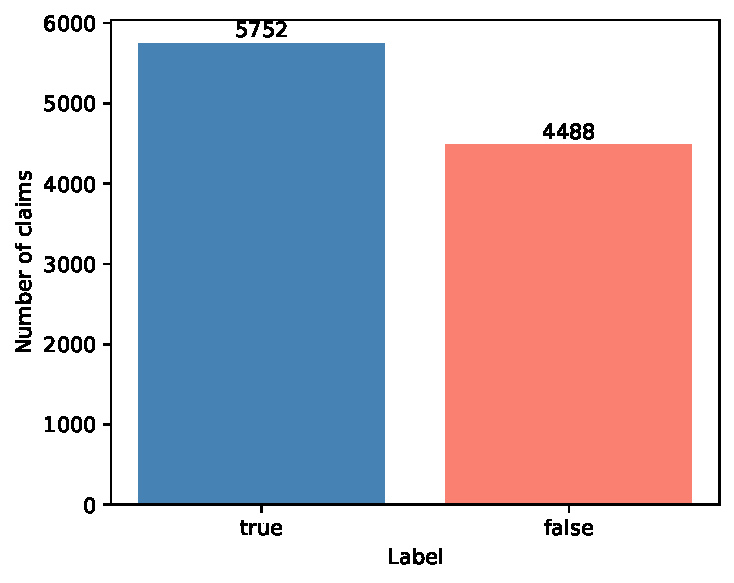
\includegraphics[width=0.7\textwidth]{Bilder/label_distribution_binary_train.pdf}
    \caption{Binary label distribution in the LIAR training set after mapping the 
    original six-class labels to true and false. The dataset exhibits a moderate 
    class imbalance, with true labels accounting for approximately 56\% of training 
    instances.}
    \label{fig:liar_label_distribution}
\end{figure}

\section{Task Definition}

This section defines the learning tasks addressed in this thesis and clarifies the modeling assumptions underlying the experimental setup. In particular, it distinguishes between binary and multi-class classification settings and introduces the notion of domain-aware versus domain-agnostic modeling, which plays a central role in the proposed agent-based framework.

\subsection{Binary vs. Multi-Class Classification}

Fake news and fact-checking tasks can be formulated in different ways depending on the target label space. Multi-class classification aims to predict fine-grained truthfulness labels, such as multiple degrees of factual correctness. While this formulation provides detailed output, it is also significantly more challenging due to class imbalance, annotation subjectivity, and limited training data for minority classes \cite{henning-etal-2023-survey}.

In this thesis, the task is formulated as a binary classification problem, where each claim is labeled as either true or false. This formulation aligns with many real-world fact-checking scenarios, where the primary objective is to distinguish factual from non-factual information \cite{vykopal2024generativelargelanguagemodels}. Binary classification also enables a more controlled evaluation of model behavior and facilitates fair comparison between different system configurations.

Rather than focusing on fine-grained truthfulness prediction, this thesis emphasizes the interaction between agents and domain information. Restricting the task to binary classification allows the analysis to concentrate on the impact of domain awareness and agent collaboration, without confounding effects introduced by highly imbalanced multi-class labels.

\subsection{Domain-Aware vs. Domain-Agnostic Settings}

Beyond the choice of label space, this thesis distinguishes between domain-aware and domain-agnostic modeling settings. In a domain-agnostic setting, the model receives only the claim text as input and must implicitly infer any relevant domain information during prediction. This reflects a standard classification setup commonly used in prior work \cite{schulhoff2025promptreportsystematicsurvey}.

In contrast, a domain-aware setting explicitly incorporates domain information into the decision process. In this thesis, domain knowledge is not derived from external sources, databases, or retrieval systems. Rather, it is operationalized exclusively through two mechanisms that rely on information already present in the LIAR dataset:

\begin{itemize}
    \item \textbf{Subject metadata as context:} The LIAR dataset provides 
    human-annotated subject tags for each statement (e.g., 
    \textit{health-care}, \textit{taxes}, \textit{elections}). These tags 
    are optionally prepended to the prompt as additional context, allowing 
    the model to leverage topical cues present in the dataset metadata.
    
    \item \textbf{Domain-specialized agents:} In the multi-agent framework, 
    claims are routed to domain-specific expert agents that have been 
    fine-tuned on domain-restricted subsets of the training data. These 
    agents implicitly encode domain knowledge through their training 
    distribution rather than through external information retrieval.
\end{itemize}

Consequently, domain awareness in this thesis refers to the structured use of existing dataset metadata and training signal. This design ensures full reproducibility and enables direct comparability with prior work on the same benchmark.

\section{Problem Setup Overview}

Figure~\ref{fig:pipeline_overview} illustrates the setup used in this thesis. Each input consists of a short political claim from the LIAR dataset, optionally accompanied by human-annotated subject tags. After preprocessing, the claim is passed to a 
classification system -- either a single LLM or a multi-agent pipeline -- which produces a binary verdict (\texttt{True} or 
\texttt{False}).

\begin{figure}[htbp]
\centering
\begin{tikzpicture}[
    box/.style={rectangle, rounded corners=3pt, draw, minimum width=4.5cm,
                minimum height=1.0cm, align=center, font=\small},
    data/.style={box, fill=orange!20, draw=orange!60},
    process/.style={box, fill=blue!15, draw=blue!50},
    optional/.style={box, fill=gray!15, draw=gray!50, dashed},
    output/.style={box, fill=green!20, draw=green!60},
    arrow/.style={-{Stealth}, thick},
]

\node[data] (dataset) at (0, 0) {
    \textbf{LIAR Dataset}\\
    \footnotesize short political claims};

\node[process] (preproc) at (0, -2) {
    \textbf{Preprocessing}\\
    \footnotesize text cleaning\\
    \footnotesize binary label mapping\\
    \footnotesize domain label mapping};

\node[optional] (subjects) at (5.5, -4) {
    \textbf{Subject Tags}\\
    \footnotesize (optional domain context)};

\node[process] (model) at (0, -4) {
    \textbf{Classification System}\\
    \footnotesize Single LLM or Multi-Agent};

\node[output] (verdict) at (0, -5.5) {
    \textbf{Binary Verdict}\\
    \footnotesize \texttt{True} / \texttt{False}};

\draw[arrow] (dataset) -- (preproc);
\draw[arrow] (preproc) -- (model);
\draw[arrow, dashed] (subjects) -- (model);
\draw[arrow] (model) -- (verdict);

\node[align=left, font=\footnotesize, text=gray] at (5.5, -0.0) {
    \textit{``The unemployment rate is}\\
    \textit{at a 50-year low.''}};

\draw[->, gray, dashed] (3.2, -0.0) -- (dataset.east);

\end{tikzpicture}
\caption{Overview of the binary claim verification setup. Each short political claim from the LIAR dataset is preprocessed and passed to a classification system, optionally augmented with human-annotated subject tags. The system outputs a binary verdict 
(\texttt{True}/\texttt{False}).}
\label{fig:pipeline_overview}
\end{figure}

